% XeLaTeX can use any Mac OS X font. See the setromanfont command below.
% Input to XeLaTeX is full Unicode, so Unicode characters can be typed directly into the source.

% The next lines tell TeXShop to typeset with xelatex, and to open and save the source with Unicode encoding.

%!TEX TS-program = xelatex
%!TEX encoding = UTF-8 Unicode

\documentclass[12pt]{article}
\usepackage{geometry}                % See geometry.pdf to learn the layout options. There are lots.
\geometry{letterpaper}                   % ... or a4paper or a5paper or ... 
%\geometry{landscape}                % Activate for for rotated page geometry
%\usepackage[parfill]{parskip}    % Activate to begin paragraphs with an empty line rather than an indent
\usepackage{graphicx}
\usepackage{amssymb}
\usepackage{verbatim}
% Will Robertson's fontspec.sty can be used to simplify font choices.
% To experiment, open /Applications/Font Book to examine the fonts provided on Mac OS X,
% and change "Hoefler Text" to any of these choices.

\usepackage{fontspec,xltxtra,xunicode}
\defaultfontfeatures{Mapping=tex-text}
\setromanfont[Mapping=tex-text]{Hoefler Text}
\setsansfont[Scale=MatchLowercase,Mapping=tex-text]{Gill Sans}
\setmonofont[Scale=MatchLowercase]{Andale Mono}

\title{Project report for COMP5221}
\author{MAO Zhili 20169034}
%\date{}                                           % Activate to display a given date or no date

\begin{document}
\maketitle
\section{Project proposal}
Translating ``pinyin'' into right Chinese sentences.
\begin{enumerate} 
\item
Create a very large parallel corpus where Language 0 is real Chinese character sentences, and Language 1 is the corresponding pinyin sentences.  This would be easy to produce automatically, since you could automatically produce pinyin given Chinese character text.
\item
Get as large as possible a dictionary of Chinese-characters-to-pinyin.  
These two together would be the training corpus, and could be directly submitted to SMT training.
\end{enumerate}
\section{Method}
I assume the ``pinyin'' is a sequence of observations and the Chinese characters is a sequence of output. Between them the POS-tag is the hiden states. 
Besides the dictionary of Chinese-characters-to-pinyin, I used a corpus of the Chinese-vocabulary with POS-tag to built the pinyin-POStag-pinyin-Chinese model. In this model I have four Matrix as the defult input. 
\begin{enumerate}
\item
Transition\_matrix: This matrix stores the transition probability of transiting from state to state, in another word, tag to tag.
\item
Initial\_matrix: This matrix stores the probability of a certain state is the first state in a sentence.
\item
Emission\_matrix: This matrix stores the probability of a certain observing to a certain state.
\item 
Vocabulary\_matrix: This matrix stores the probability of a certain observing to a certain output Chinese. 
\end{enumerate}
The main task of this project is using Viterbi algorithm to segment the a sequence of observations what is discussed in the tutorial. The raw structure shows as fig.\ref{fig:structure}
\begin{figure}[htp]
	\centering
	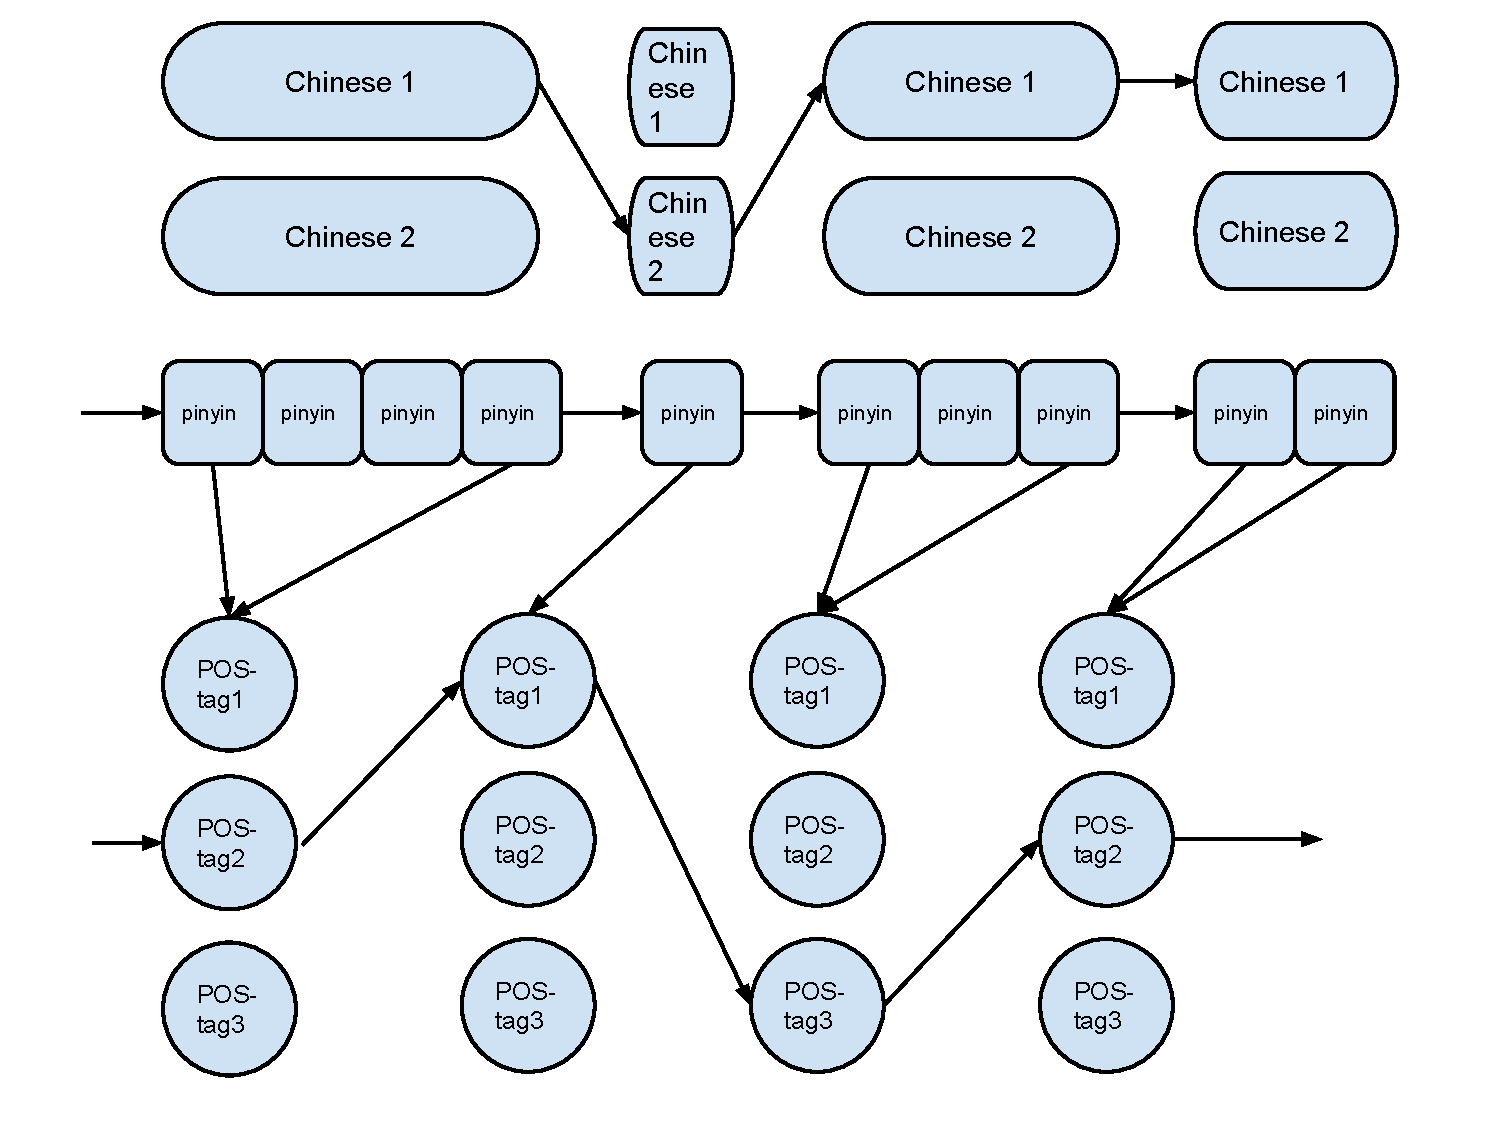
\includegraphics[width=0.8\textwidth]{py2tag2chinese.pdf}
	\caption{Structure}
	\label{fig:structure}
\end{figure}

\section{Result}
The result is not very good. I guess it is due to the corpus.
Run the demo.py and demo2.py could see the result. 
\section{Future work}
\begin{enumerate}
\item
Numbers and punctuation mark need to be considered.
\item
More test and program improve to get the statistical result of this model.
\item
Improve the model with new corpus or the algorithm.
\end{enumerate}
\end{document}  
